\subsection{Zookeeper}
\label{sec:zookeeper}
ZooKeeper è un servizio, centralizzato e open source, di coordinamento affidabile per applicazioni distribuite \cite{zookeeper:home}. I servizi di coordinamento sono notoriamente difficili da ottenere; sono, infatti, particolarmente inclini a errori derivanti, ad esempio, da condizioni di stallo. ZooKeeper, invece, fornisce servizi operativi per cluster di grandi dimensioni. Esempi di questi servizi includono: informazioni di configurazione distribuita, un servizio di sincronizzazione e un registro di denominazione per i sistemi distribuiti. Le applicazioni sfruttano questi servizi per coordinare l'elaborazione distribuita tra cluster di grandi dimensioni. ZooKeeper inoltre, mira a semplificare la natura di questi diversi servizi in un'interfaccia molto semplice creando un servizio di coordinamento centralizzato. Il servizio stesso è distribuito e altamente affidabile. Questo perché, questo tipo di servizi risulta essere di difficile implementazione per le applicazioni distribuite.
\\Lo spazio dei nomi è costituito da registri di dati, chiamati znodes, in linguaggio ZooKeeper, che sono simili ai file e alle directory. A differenza di un tipico file system, progettato per l'archiviazione, i dati di ZooKeeper vengono conservati in memoria, il che significa che ZooKeeper può ottenere alti throughput e bassi numeri di latenza. Il database replicato di ZooKeeper comprende un albero di znodi, entità che rappresentano approssimativamente i nodi del file system (simili a directory). Ogni znode può essere arricchito da una matrice di byte, che memorizza i dati. Inoltre, ogni znode può avere altri znodi sotto di esso, praticamente formando un sistema di directory interno.
\\Zookeeper è considerato un servizio robusto, dal momento che i dati persistenti sono distribuiti tra più nodi (questo insieme di nodi è chiamato "ensemble") e un client si connette a uno di essi (cioè un "server" specifico), migrando se un nodo fallisce; Finché funziona la stragrande maggioranza dei nodi, l'insieme dei nodi ZooKeeper è vivo. In particolare, un nodo master viene scelto dinamicamente per consenso all'interno dell'ensemble; se il nodo principale non funziona, il ruolo del master passa a un altro nodo. È interessante notare che il nome di uno znode può essere sequenziale, il che significa che il nome che il client fornisce quando si crea lo znode è solo un prefisso: il nome completo è dato anche da un numero sequenziale scelto dall'ensemble. Ciò è utile, ad esempio, per scopi di sincronizzazione: se più client desiderano ottenere un blocco su una risorsa, possono contemporaneamente creare uno znode sequenziale su una posizione: chi ottiene il numero più basso ha diritto al blocco.
\\Inoltre, uno znode può essere “effimero” (temporaneo): questo significa che viene distrutto non appena il client che lo ha creato si disconnette. Ciò è utile soprattutto per sapere quando un client fallisce, il che può essere rilevante quando il client stesso ha delle responsabilità che dovrebbero essere prese da un nuovo client. Tutte le richieste di scrittura dei client vengono inoltrate a un singolo server, chiamato leader: in questo modo è possibile garantire che le scritture siano mantenute in ordine, vale a dire che le scritture siano lineari. Il resto dei server ZooKeeper, chiamati follower, riceve proposte di messaggi dal leader e concorda la consegna dei messaggi. Il livello di messaggistica si occupa di sostituire i leader in caso di fallimento e di sincronizzare i follower con il leader. ZooKeeper utilizza un protocollo di messaggistica atomica personalizzato. Poiché il livello di messaggistica è atomico, ZooKeeper può garantire che le repliche locali non divergano mai. Quando il leader riceve una richiesta di scrittura, calcola lo stato del sistema quando deve essere applicata la scrittura e lo trasforma in una transazione che cattura questo nuovo stato.
\\Ogni volta che un client scrive sull'ensemble, la maggior parte dei nodi mantiene l'informazione: questi nodi includono il server per il client e ovviamente il leader. Ciò significa che ogni scrittura rende il server aggiornato con il leader. Significa anche, tuttavia, che non è possibile avere scritture simultanee. La garanzia delle scritture lineari è la ragione del fatto che ZooKeeper non offra prestazioni ottimali per i carichi di lavoro dominanti dalla scrittura. In particolare, non dovrebbe essere usato per l'interscambio di grandi dati, come i media. Fintanto che la comunicazione coinvolga dati condivisi, ZooKeeper è utile. Quando i dati possono essere scritti contemporaneamente, ZooKeeper interviene, perché impone un rigoroso ordine di operazioni anche se non strettamente necessario dal punto di vista di chi scrive. Per la lettura, invece, ZooKeeper eccelle, questo perché le letture sono simultanee poiché sono servite dallo specifico server al quale il client si connette.
\begin{figure}[H]
\centering
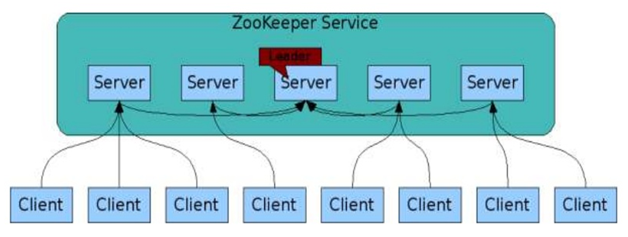
\includegraphics[width=\textwidth]{./images/zookeeper.png}
\caption{Funzionamento di Zookeeper.}
\label{fig:zookeeper}
\end{figure}
ZooKeeper, in sintesi, è servizio molto veloce e molto semplice. La velocità di zookeeper è data da carichi di lavoro in cui le letture dei dati sono più comuni delle scritture. Il rapporto di lettura / scrittura ideale è di circa 10:1. Inoltre, Zookeeper mantiene uno spazio dei nomi gerarchico standard, simile a file e directory, questo lo rende un sistema sostanzialmente semplice. ZooKeeper viene replicato su un insieme di host (chiamato “ensemble”) e i server sono a conoscenza l'uno dell'altro. Finché sarà disponibile una massa critica di server, sarà disponibile anche il servizio ZooKeeper. Non c'è un singolo punto di errore. Per questo Zookeeper è detto: affidabile.
\\Dal momento che il suo obiettivo, però, è quello di essere una base per la costruzione di servizi più complicati, come la sincronizzazione, fornisce un insieme di garanzie tra cui:
\begin{itemize}
\item \textit{Consistenza sequenziale}: gli aggiornamenti da un client verranno applicati nell'ordine in cui sono stati inviati.
\item \textit{Atomicità}: gli aggiornamenti hanno esito positivo o negativo. Nessun risultato parziale.
\item \textit{Immagine del sistema singolo}: un client vedrà la stessa vista del servizio indipendentemente dal server a cui si connette.
\item \textit{Affidabilità}: una volta applicato un aggiornamento, esso persisterà da quel momento fino a quando un client non sovrascriverà l'aggiornamento.
\item \textit{Tempestività}: la visualizzazione dei client del sistema è garantita per essere aggiornata entro un certo limite di tempo.
\end{itemize}

\subsubsection{Kafka}
\label{sec:kafka}
Apache Kafka è una piattaforma di streaming open source distribuita che può essere utilizzata per compilare applicazioni e pipeline di dati in streaming in tempo reale. Kafka offre anche una funzionalità di broker di messaggi simile a una coda di messaggi, dove è possibile pubblicare e sottoscrivere flussi dei dati denominati \cite{kafka:microsoft}. Apache Kafka permette la gestione di centinaia di megabyte di traffico in lettura e scrittura al secondo da parte migliaia di Client. È stato sviluppato per la prima volta su LinkedIn e viene spesso utilizzato in combinazione con Apache Spark Streaming per l'elaborazione dei flussi in tempo reale.
\\Kafka ha un'architettura che differisce significativamente da altri sistemi di messaggistica. Ogni nodo prende il nome di broker. Kafka offre un'API Producer per la pubblicazione di record in un topic Kafka e un’API Consumer che viene utilizzata quando si sottoscrive un topic. Un topic è un nome di categoria o feed a cui i record sono pubblicati. I Topic in Kafka sono sempre multi-abbonato; cioè, un argomento può avere zero, uno o più consumatori che si abbonano ai dati scritti su di esso \cite{kafka:home}. Kafka archivia i record in topic. Un topic è un insieme di messaggi della stessa categoria; per ogni topic il cluster Kafka mantiene un registro partizionato. Ogni partizione è una sequenza ordinata ed immutabile di messaggi che vengono aggiunti in continuazione all’interno del registro. I record, che come abbiamo visto sono archiviati in topic, vengono prodotti da un producer e usati dai consumer. I Producers o produttori pubblicano i messaggi (i dati) all’interno di un topic. Il Producer è responsabile di scegliere in quale partizione del registro del topic inserire un proprio messaggio. Ogni Producer sceglie il proprio algoritmo di assegnamento (per esempio un semplice round robin). I Consumers o consumatori leggono (consumano) i dati presenti all’interno del topic. Nel caso del sistema distribuito il produttore è integrato nell'ecosistema Spark, mentre il consumatore è una libreria creata ad-hoc presente all'interno della Webapp, in particolare nell'ecosistema NodeJS. 
\\Ogni partizione è una sequenza ordinata e immutabile di record che viene continuamente aggiunta a un registro di commit strutturato. Ai record nelle partizioni viene assegnato un numero ID sequenziale chiamato offset che identifica in modo univoco ogni record all'interno della partizione \cite{kafka:home}.
\\In Kafka le partizioni sono replicate tra i nodi per garantire protezione in caso di interruzioni dei nodi (broker). La replicazione di una partizione viene gestita automaticamente in modo che sia assegnata a diversi brokers. Kafka elegge per ogni Broker una partizione “Leader” (indicato con (L)) e tutte le scritture e le letture dovranno passare alla partizione “Leader” scelta. Il traffico dei producer viene indirizzato al leader di ogni nodo, usando lo stato gestito da ZooKeeper. 
\begin{figure}[H]
\centering
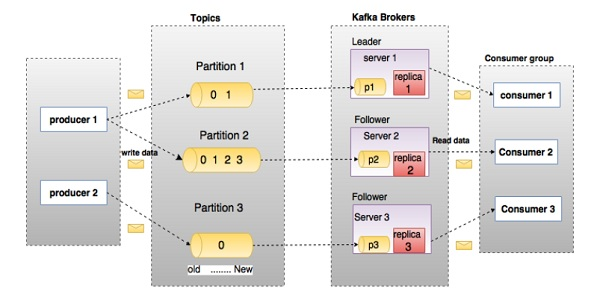
\includegraphics[width=\textwidth]{./images/kafkaArchitetture.jpg}
\caption{Come funziona Kafka}
\label{fig:clusterKafka}
\end{figure}
Infine, la messaggistica in Kafka prevede solo due di tipi di modelli: 
\begin{itemize}
\item \textit{Queuing (Coda)}: un pool di Consumers può leggere dal Server e ciascuno può leggere i dati solamente durante il suo turno; 
\item \textit{Publish - subscribe}: il messaggio viene trasmesso a tutti i Consumers. 
\end{itemize}
Kafka offre una sola implementazione dell'entità Consumer che generalizza entrambi i modelli, il consumer group.  Un Consumer etichetta se stesso con il nome del gruppo a cui decide di far parte e ciascun messaggio pubblicato in un topic, seguito dal gruppo, viene consegnato a ciascun Consumer presente.  Se tutti i Consumer hanno lo stesso consumer group, il sistema si reduce ad una semplice coda con priorità first in - first out (FIFO).  Se tutti i consumer hanno un consumer group diverso, il sistema automaticamente diventa di tipo publish-subscribe.